\documentclass{article}
\setlength{\parindent}{0pt}
\setlength{\parskip}{2ex plus 0.5ex minus 0.2ex}
\usepackage[margin=1in]{geometry}
\usepackage{graphicx}
\usepackage{hyperref}
\usepackage{cleveref}
\graphicspath{{./figures/}}

\begin{document}

\section{Comprehensive, expensive (3D) models}

\subsection{MSBR}

The most detailed report on ORNL's molten salt breeder reactor is the technical
report by Robertson. \cite{robertson_conceptual_1971} A nice overview of the
MSBR geometry is shown in \cref{fig:vertical,fig:horizontal,fig:zoom_horiz}.

\begin{figure}[htpb]
  \centering
  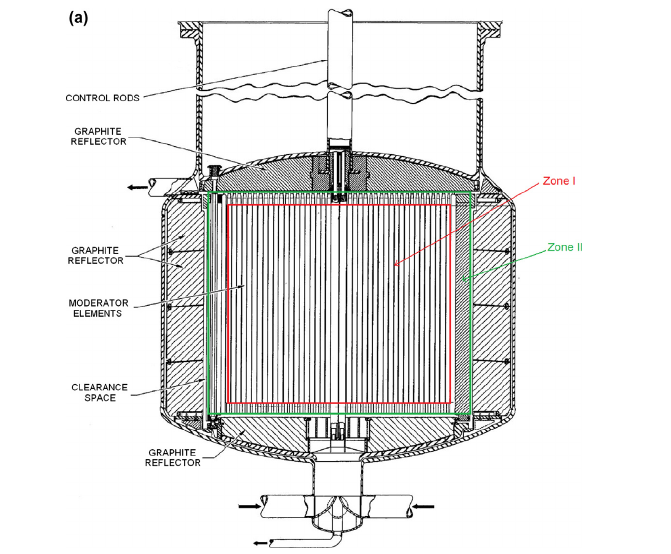
\includegraphics{vertical_MSBR_cross_section.png}
  \caption{Vertical cross section of MSBR.}
  \label{fig:vertical}
\end{figure}
\begin{figure}[htpb]
  \centering
  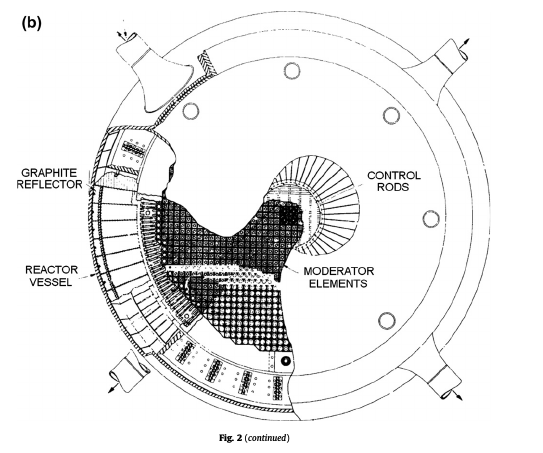
\includegraphics{horizontal_MSBR_cross_section.png}
  \caption{Horizontal cross section of MSBR.}
  \label{fig:horizontal}
\end{figure}
\begin{figure}[htpb]
  \centering
  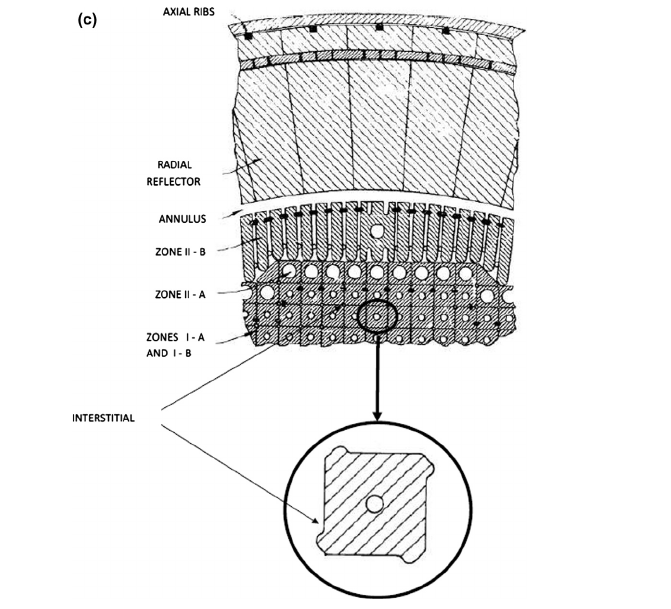
\includegraphics{zoomed_horizontal_MSBR_cross_section.png}
  \caption{Zoomed in horizontal cross-section of MSBR. Shows presence of
    interstitials between graphite block elements in zone 1 of the reactor.}
  \label{fig:zoom_horiz}
\end{figure}

\section{Simplified models}

\subsection{MSBR children}

\subsubsection{Cammi et. al.}

This model is based on the multi-physics model by
\cite{cammi_multi-physics_2011}.

\bibliographystyle{unsrt}
\bibliography{MSR-design}
\end{document}
